\chapter{Motivation and Approach}

\section{Adaptive sampling: Motivation}
Physical systems come in many forms and shapes and 

Intrinsic hierachical organisation

Molecular dynamics (MD) simulations have become indispensable for gaining
insight into molecular systems at high spatial and temporal resolutions.
However, a key limitation for MD with accurate all-atom force-fields remains
the computational demand for simulating processes with long timescales. In
particular, biologically relevant processes, such as protein folding and
conformational changes, typically require simulation time in excess of
milliseconds, while atomic-resolution MD trajectories can currently reach
timescales on the order of microseconds on standard computational resources. 



This thesis is about solving the challenge of accurately determining the confomational dynamics of high-dimensional stochastic systems. This challenge of high-dimensional stochastic dynamics   
adaptive sampling of conformational dynamics, a method to efficiently obtain relevant information about the stationary and kinetic behavior of high-dimensional stochastic dynamics. This methods is especially usefull in the context of molecular dynamics (MD) of proteins. Proteins and the obtaining of accurate stationary and kinetic behavior of protein is a crucial unsolved challenge which limits our understanding of the behavior of many systems. This includes the majority of biological processes.
\RED{expand}
adaptive sampling is one layer on top 
of other tool. such as dimension reduction



\section{Outline}
 
Overall this Dissertation resulted in several peer-reviewed publications \cite{Adstrategies2018, Extasy2016}, as well one publication under review \cite{Extasy2019}. The results obtained during my dissertation as well the results in the papers will be presented in the next chapters.
 
Chapter \label{sec:background} will summarize some of the standard techniques, which will be used frequently throughout the thesis. While some of these approaches are commonly used in this field, there are also recently developed techniques which are less commonly used. The relevence of all these techniques for adaptive sampling will be highlighted. 

The theory of Adaptive sampling will be discussed in Chapter \label{ch:chapter3}, as well the derivation of the first upper limit of the adaptive sampling speed up will be show. This novel result shows that adaptive sampling can be further improved. 
In the next chapter \label{ch:chapter32} the current strategies will be compared in statistically robust way and the effectivity of each strategy will be compared for different proteins and different goals.

Chapter \label{ch:chapter4} will introduce the computational tools and software frame works necessary to successfully and efficiently execute adaptive sampling. Due to the many subtasks adaptive sampling consists off, these practical consideration have a direct impact on the viability of adaptive sampling for solving sampling problems.

This developed software framework will be used in Chapter \label{ch:chapter5} to show for different biomolecular systems the results and the accuracy which adaptive sampling can achieve. 

A final chapter \label{ch:conclude} will summarize the current achievements and discuss further open questions and possible directions.


\afterpage{\null\newpage}
\chapter{Background\label{sec:background}}

\section{Biomolecules}

\GRE{ 
The behavior of a protein or any biomolecule can be represented by the xyz positions and velocities of all the . T}
\RED{nice pic protein disease}


\section{Proteins and Molecular Dynamics (MD)}
\label{sec:MD}
\GRE{ The behavior of a protein or any biomolecule can be represented by the xyz positions and velocities of all the . T}
\RED{ image protein xyz}
check lorenzo chapter 1

The standard tool to access all of this information is Molecular Dynamics (MD), which is
the science of simulating motion of a system of particles according to Newton’s classical
equations of motion.
The time evolution of a system of N atoms obeys the following Cauchy problem:

X 2 R3N denotes the full Cartesian vector of the system


$$M\ddot{X_{t}}=-\nabla U(x_{t})$$

$$U_{CHARMM}=U_{bonds}+U_{angle}+U_{dihedral}+U_{improper}+U_{UB}+U_{LJ}+U_{elec}$$

equation for charmm22
\begin{equation}
\begin{aligned}
U(r_{i})={} &\sum_{bonds}K_{b}(b-b_{0})^{2}+\sum_{angles}K_{\theta}(\theta-\theta_{0})^{2}+\sum_{torsions}K_{\phi}\left(1+cos(n\phi-\delta)\right)\\
&+\sum_{impropers}k_{\omega}\left(\omega-\omega_{0}\right)^{2}+\sum_{Urey-Bradley}k_{u}\left(u-u_{0}\right)^{2}\\
&+\sum_{nonbonded}\epsilon\left[\left(\frac{R_{min,ij}}{r_{ij}}\right)^{12}-\left(\frac{R_{min,ij}}{r_{ij}}\right)^{6}\right]+\sum_{electric}\frac{q_{i}q_{j}}{\epsilon r_{ij}}
\end{aligned}
\end{equation}

The graphics cards can currently simulate almost 1 microsecond of MD trajectory per day of simulation time for smaller proteins. The Special purpose hardware can simulate up to 100 microseconds of MD trajectory per simulation day, but the major limitation of the special-purpose hardware is the very limited access to these machines. 

\section{TICA}
dimension reduction
check  lorenzo chapter 2
page 188, b./3

scale sqaure rrot

koppman approcimation


Time-lagged Independent Component Analysis (TICA) [100, 109, 110] is a dimensionality
reduction method that can be considered as a special case of the application of the
variational principle presented above. In practice, given MD data, TICA performs a variational
optimization using a set of input molecular features yi(xt) (such as atomic positions,
distances, dihedral angles and combinations of those, . . . ) and defining mean-free basis
functions as
$$f_{t}=F\left(x_{t}-\left\langle x_{t}\right\rangle \right)$$
These

variational principle for conformational dynamics (VAC)


\section{vampnet intro}
vampnet intro


xy trajectory
$$x_{t}$$

features
$$f_{t}$$

dimension reduced trajeory

$$o_{t}$$

$$C_{01}=\ensuremath{\mathbb{E}}_{t}\left[o_{t}o_{t+\tau}\right]$$
loss function
$$L=\left\Vert C_{00}^{-1/2}C_{01}C_{11}^{-1/2}\right\Vert ^{2}$$

\begin{figure}[h]
  \centering
  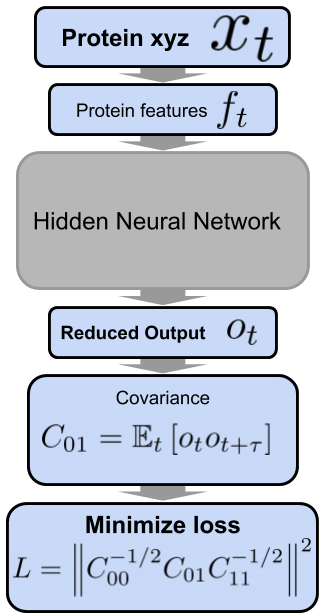
\includegraphics[width=0.4\linewidth]{figures3/NN.png}
  \caption{NN}
  \label{fig:NN}
\end{figure}


crossvalidation  - lorenzo fig5 6.1


\section{MSM}
check  lorenzo chapter 2
mfpt
eigenvectors

markovian property

implied timescales equation 3.12

\section{energy landscape }
energy landscape 
folding funnel
focker planck equation

Boltzmann distribution - lornezo
lronzeo fig 7.6

state space


[12]